\documentclass[12pt,a4paper]{article}

\usepackage[a4paper,text={16.5cm,25.2cm},centering]{geometry}
\usepackage{lmodern}
\usepackage{amssymb,amsmath}
\usepackage{bm}
\usepackage{graphicx}
\usepackage{microtype}
\usepackage{hyperref}
\setlength{\parindent}{0pt}
\setlength{\parskip}{1.2ex}

\hypersetup
       {   pdfauthor = { Marco Fasondini },
           pdftitle={ foo },
           colorlinks=TRUE,
           linkcolor=black,
           citecolor=blue,
           urlcolor=blue
       }




\usepackage{upquote}
\usepackage{listings}
\usepackage{xcolor}
\lstset{
    basicstyle=\ttfamily\footnotesize,
    upquote=true,
    breaklines=true,
    breakindent=0pt,
    keepspaces=true,
    showspaces=false,
    columns=fullflexible,
    showtabs=false,
    showstringspaces=false,
    escapeinside={(*@}{@*)},
    extendedchars=true,
}
\newcommand{\HLJLt}[1]{#1}
\newcommand{\HLJLw}[1]{#1}
\newcommand{\HLJLe}[1]{#1}
\newcommand{\HLJLeB}[1]{#1}
\newcommand{\HLJLo}[1]{#1}
\newcommand{\HLJLk}[1]{\textcolor[RGB]{148,91,176}{\textbf{#1}}}
\newcommand{\HLJLkc}[1]{\textcolor[RGB]{59,151,46}{\textit{#1}}}
\newcommand{\HLJLkd}[1]{\textcolor[RGB]{214,102,97}{\textit{#1}}}
\newcommand{\HLJLkn}[1]{\textcolor[RGB]{148,91,176}{\textbf{#1}}}
\newcommand{\HLJLkp}[1]{\textcolor[RGB]{148,91,176}{\textbf{#1}}}
\newcommand{\HLJLkr}[1]{\textcolor[RGB]{148,91,176}{\textbf{#1}}}
\newcommand{\HLJLkt}[1]{\textcolor[RGB]{148,91,176}{\textbf{#1}}}
\newcommand{\HLJLn}[1]{#1}
\newcommand{\HLJLna}[1]{#1}
\newcommand{\HLJLnb}[1]{#1}
\newcommand{\HLJLnbp}[1]{#1}
\newcommand{\HLJLnc}[1]{#1}
\newcommand{\HLJLncB}[1]{#1}
\newcommand{\HLJLnd}[1]{\textcolor[RGB]{214,102,97}{#1}}
\newcommand{\HLJLne}[1]{#1}
\newcommand{\HLJLneB}[1]{#1}
\newcommand{\HLJLnf}[1]{\textcolor[RGB]{66,102,213}{#1}}
\newcommand{\HLJLnfm}[1]{\textcolor[RGB]{66,102,213}{#1}}
\newcommand{\HLJLnp}[1]{#1}
\newcommand{\HLJLnl}[1]{#1}
\newcommand{\HLJLnn}[1]{#1}
\newcommand{\HLJLno}[1]{#1}
\newcommand{\HLJLnt}[1]{#1}
\newcommand{\HLJLnv}[1]{#1}
\newcommand{\HLJLnvc}[1]{#1}
\newcommand{\HLJLnvg}[1]{#1}
\newcommand{\HLJLnvi}[1]{#1}
\newcommand{\HLJLnvm}[1]{#1}
\newcommand{\HLJLl}[1]{#1}
\newcommand{\HLJLld}[1]{\textcolor[RGB]{148,91,176}{\textit{#1}}}
\newcommand{\HLJLs}[1]{\textcolor[RGB]{201,61,57}{#1}}
\newcommand{\HLJLsa}[1]{\textcolor[RGB]{201,61,57}{#1}}
\newcommand{\HLJLsb}[1]{\textcolor[RGB]{201,61,57}{#1}}
\newcommand{\HLJLsc}[1]{\textcolor[RGB]{201,61,57}{#1}}
\newcommand{\HLJLsd}[1]{\textcolor[RGB]{201,61,57}{#1}}
\newcommand{\HLJLsdB}[1]{\textcolor[RGB]{201,61,57}{#1}}
\newcommand{\HLJLsdC}[1]{\textcolor[RGB]{201,61,57}{#1}}
\newcommand{\HLJLse}[1]{\textcolor[RGB]{59,151,46}{#1}}
\newcommand{\HLJLsh}[1]{\textcolor[RGB]{201,61,57}{#1}}
\newcommand{\HLJLsi}[1]{#1}
\newcommand{\HLJLso}[1]{\textcolor[RGB]{201,61,57}{#1}}
\newcommand{\HLJLsr}[1]{\textcolor[RGB]{201,61,57}{#1}}
\newcommand{\HLJLss}[1]{\textcolor[RGB]{201,61,57}{#1}}
\newcommand{\HLJLssB}[1]{\textcolor[RGB]{201,61,57}{#1}}
\newcommand{\HLJLnB}[1]{\textcolor[RGB]{59,151,46}{#1}}
\newcommand{\HLJLnbB}[1]{\textcolor[RGB]{59,151,46}{#1}}
\newcommand{\HLJLnfB}[1]{\textcolor[RGB]{59,151,46}{#1}}
\newcommand{\HLJLnh}[1]{\textcolor[RGB]{59,151,46}{#1}}
\newcommand{\HLJLni}[1]{\textcolor[RGB]{59,151,46}{#1}}
\newcommand{\HLJLnil}[1]{\textcolor[RGB]{59,151,46}{#1}}
\newcommand{\HLJLnoB}[1]{\textcolor[RGB]{59,151,46}{#1}}
\newcommand{\HLJLoB}[1]{\textcolor[RGB]{102,102,102}{\textbf{#1}}}
\newcommand{\HLJLow}[1]{\textcolor[RGB]{102,102,102}{\textbf{#1}}}
\newcommand{\HLJLp}[1]{#1}
\newcommand{\HLJLc}[1]{\textcolor[RGB]{153,153,119}{\textit{#1}}}
\newcommand{\HLJLch}[1]{\textcolor[RGB]{153,153,119}{\textit{#1}}}
\newcommand{\HLJLcm}[1]{\textcolor[RGB]{153,153,119}{\textit{#1}}}
\newcommand{\HLJLcp}[1]{\textcolor[RGB]{153,153,119}{\textit{#1}}}
\newcommand{\HLJLcpB}[1]{\textcolor[RGB]{153,153,119}{\textit{#1}}}
\newcommand{\HLJLcs}[1]{\textcolor[RGB]{153,153,119}{\textit{#1}}}
\newcommand{\HLJLcsB}[1]{\textcolor[RGB]{153,153,119}{\textit{#1}}}
\newcommand{\HLJLg}[1]{#1}
\newcommand{\HLJLgd}[1]{#1}
\newcommand{\HLJLge}[1]{#1}
\newcommand{\HLJLgeB}[1]{#1}
\newcommand{\HLJLgh}[1]{#1}
\newcommand{\HLJLgi}[1]{#1}
\newcommand{\HLJLgo}[1]{#1}
\newcommand{\HLJLgp}[1]{#1}
\newcommand{\HLJLgs}[1]{#1}
\newcommand{\HLJLgsB}[1]{#1}
\newcommand{\HLJLgt}[1]{#1}



\def\qqand{\qquad\hbox{and}\qquad}
\def\qqfor{\qquad\hbox{for}\qquad}
\def\qqas{\qquad\hbox{as}\qquad}
\def\half{ {1 \over 2} }
\def\D{ {\rm d} }
\def\I{ {\rm i} }
\def\E{ {\rm e} }
\def\C{ {\mathbb C} }
\def\R{ {\mathbb R} }
\def\H{ {\mathbb H} }
\def\Z{ {\mathbb Z} }
\def\CC{ {\cal C} }
\def\FF{ {\cal F} }
\def\HH{ {\cal H} }
\def\LL{ {\cal L} }
\def\vc#1{ {\mathbf #1} }
\def\bbC{ {\mathbb C} }



\def\fR{ f_{\rm R} }
\def\fL{ f_{\rm L} }

\def\qqqquad{\qquad\qquad}
\def\qqwhere{\qquad\hbox{where}\qquad}
\def\Res_#1{\underset{#1}{\rm Res}\,}
\def\sech{ {\rm sech}\, }
\def\acos{ {\rm acos}\, }
\def\asin{ {\rm asin}\, }
\def\atan{ {\rm atan}\, }
\def\Ei{ {\rm Ei}\, }
\def\upepsilon{\varepsilon}


\def\Xint#1{ \mathchoice
   {\XXint\displaystyle\textstyle{#1} }%
   {\XXint\textstyle\scriptstyle{#1} }%
   {\XXint\scriptstyle\scriptscriptstyle{#1} }%
   {\XXint\scriptscriptstyle\scriptscriptstyle{#1} }%
   \!\int}
\def\XXint#1#2#3{ {\setbox0=\hbox{$#1{#2#3}{\int}$}
     \vcenter{\hbox{$#2#3$}}\kern-.5\wd0} }
\def\ddashint{\Xint=}
\def\dashint{\Xint-}
% \def\dashint
\def\infdashint{\dashint_{-\infty}^\infty}




\def\addtab#1={#1\;&=}
\def\ccr{\\\addtab}
\def\ip<#1>{\left\langle{#1}\right\rangle}
\def\dx{\D x}
\def\dt{\D t}
\def\dz{\D z}
\def\ds{\D s}

\def\rR{ {\rm R} }
\def\rL{ {\rm L} }

\def\norm#1{\left\| #1 \right\|}

\def\pr(#1){\left({#1}\right)}
\def\br[#1]{\left[{#1}\right]}

\def\abs#1{\left|{#1}\right|}
\def\fpr(#1){\!\pr({#1})}

\def\sopmatrix#1{ \begin{pmatrix}#1\end{pmatrix} }

\def\endash{–}
\def\emdash{—}
\def\mdblksquare{\blacksquare}
\def\lgblksquare{\blacksquare}
\def\scre{\E}
\def\mapengine#1,#2.{\mapfunction{#1}\ifx\void#2\else\mapengine #2.\fi }

\def\map[#1]{\mapengine #1,\void.}

\def\mapenginesep_#1#2,#3.{\mapfunction{#2}\ifx\void#3\else#1\mapengine #3.\fi }

\def\mapsep_#1[#2]{\mapenginesep_{#1}#2,\void.}


\def\vcbr[#1]{\pr(#1)}


\def\bvect[#1,#2]{
{
\def\dots{\cdots}
\def\mapfunction##1{\ | \  ##1}
	\sopmatrix{
		 \,#1\map[#2]\,
	}
}
}



\def\vect[#1]{
{\def\dots{\ldots}
	\vcbr[{#1}]
} }

\def\vectt[#1]{
{\def\dots{\ldots}
	\vect[{#1}]^{\top}
} }

\def\Vectt[#1]{
{
\def\mapfunction##1{##1 \cr}
\def\dots{\vdots}
	\begin{pmatrix}
		\map[#1]
	\end{pmatrix}
} }

\def\addtab#1={#1\;&=}
\def\ccr{\\\addtab}

\def\questionequals{= \!\!\!\!\!\!{\scriptstyle ? \atop }\,\,\,}

\begin{document}

\textbf{Applied Complex Analysis (2021)}

\section{Lecture 22: Hermite polynomials}
This lecture we overview features of Hermite polynomials, some of which also apply to Jacobi polynomials.  This includes

\begin{itemize}
\item[1. ] Rodriguez formula


\item[2. ] Approximation with Hermite polynomials


\item[3. ] Eigenstates of Schrödinger equations with a quadratic well

\end{itemize}
\subsection{Rodriguez formula}
Because of the special structure of classical orthogonal weights, we have special Rodriguez formulae of the form

\[
 p_n(x) = {1 \over \kappa_n w(x)} {\D^n \over \dx^n} w(x) F(x)^n
\]
where $w(x)$ is the weight and $F(x) = (1-x^2)$ (Jacobi), $x$ (Laguerre) or $1$ (Hermite) and $\kappa_n$ is a normalization constant.

\textbf{Proposition (Hermite Rodriguez)}

\[
H_n(x)= (-1)^n \E^{x^2}  {\D^n \over \dx^n} \E^{-x^2}
\]
\textbf{Proof} We first show that it's a degree $n$ polynomial. This proceeds by induction:


\begin{align*}
 H_0(x) &= \E^{x^2} {\D^0 \over \dx^0}\E^{-x^2} = 1 \\
 H_{n+1}(x) &= -\E^{x^2}{\D \over \dx}\left[\E^{-x^2} H_{n}(x)\right] =   2x H_{n}(x) - H_n'(x)
\end{align*}
Orthogonality follows from integration by parts:

\[
\ip<H_n, p_m>_{\rm H} = (-1)^n \int_{-\infty}^{\infty}  {\D^n  \E^{-x^2} \over \dx^n} p_m \dx = \int_{-\infty}^{\infty}  \E^{-x^2} {\D^n p_m \over \dx^n} \dx = 0
\]
if $m < n$

Now we just need to show we have the right constant. But we have

\[
 {\D^n \over \dx^n}[\E^{-x^2}] =  {\D^{n-1} \over \dx^{n-1}}[-2x \E^{-x^2}] = {\D^{n-2} \over \dx^{n-2}}[(4x^2 + O(x)) \E^{-x^2}] = \cdots = \left[(-1)^n 2^n x^n + O(x^{n-1})\right]\E^{-x^2}
\]
\ensuremath{\blacksquare}

Note this tells us the Hermite recurrence: Here we have the simple expressions

\[
H_n'(x) = 2n H_{n-1}(x) \qqand {\D \over \dx}[\E^{-x^2} H_n(x)] = -\E^{-x^2} H_{n+1}(x)
\]
These follow from the same arguments as before since $w'(x) = -2x w(x)$. But using the Rodriguez formula, we get

\[
2n H_{n-1}(x)  = H_{n}'(x) = (-1)^{n} 2 x  \E^{x^2}  {\D^{n} \over \dx^{n}} \E^{-x^2}  + (-1)^n \E^{x^2}  {\D^{n+1} \over \dx^{n+1}} \E^{-x^2} = 2x H_n(x) - H_{n+1}(x)
\]
which means

\[
x H_n(x) = nH_{n-1}(x) +{H_{n+1}(x) \over 2}
\]
\subsection{Approximation with Hermite polynomials}
Hermite polynomials are typically used with the weight for approximation of functions: on the real line polynomial approximation is unnatural unless  the function approximated is a polynomial as otherwise the behaviour at \ensuremath{\infty} is inconsistent (polynomials blow up).  Thus we can either use

\[
f(x) = \E^{-x^2}\sum_{k=0}^\infty f_k H_k(x)
\]
or

\[
f(x) = \E^{-x^2/2}\sum_{k=0}^\infty f_k H_k(x)
\]
** Demonstration **

Depending on your problem, getting this wrong can be disasterous. For example, while we can certainly approximate polynomials with Hermite expansions:


\begin{lstlisting}
(*@\HLJLk{using}@*) (*@\HLJLn{ApproxFun}@*)(*@\HLJLp{,}@*) (*@\HLJLn{Plots}@*)
(*@\HLJLn{f}@*) (*@\HLJLoB{=}@*) (*@\HLJLnf{Fun}@*)(*@\HLJLp{(}@*)(*@\HLJLn{x}@*) (*@\HLJLoB{->}@*) (*@\HLJLni{1}@*)(*@\HLJLoB{+}@*)(*@\HLJLn{x}@*) (*@\HLJLoB{+}@*)(*@\HLJLn{x}@*)(*@\HLJLoB{{\textasciicircum}}@*)(*@\HLJLni{2}@*)(*@\HLJLp{,}@*) (*@\HLJLnf{Hermite}@*)(*@\HLJLp{())}@*)
(*@\HLJLnf{f}@*)(*@\HLJLp{(}@*)(*@\HLJLnfB{0.10}@*)(*@\HLJLp{)}@*)
\end{lstlisting}

\begin{lstlisting}
1.109999999999997
\end{lstlisting}


We get nonsense when trying to approximate $\sech(x)$ by a degree 50 polynomial:


\begin{lstlisting}
(*@\HLJLn{f}@*) (*@\HLJLoB{=}@*) (*@\HLJLnf{Fun}@*)(*@\HLJLp{(}@*)(*@\HLJLn{x}@*) (*@\HLJLoB{->}@*) (*@\HLJLnf{sech}@*)(*@\HLJLp{(}@*)(*@\HLJLn{x}@*)(*@\HLJLp{),}@*) (*@\HLJLnf{Hermite}@*)(*@\HLJLp{(),}@*) (*@\HLJLni{51}@*)(*@\HLJLp{)}@*)
(*@\HLJLn{xx}@*) (*@\HLJLoB{=}@*) (*@\HLJLoB{-}@*)(*@\HLJLni{8}@*)(*@\HLJLoB{:}@*)(*@\HLJLnfB{0.01}@*)(*@\HLJLoB{:}@*)(*@\HLJLni{8}@*)
(*@\HLJLnf{plot}@*)(*@\HLJLp{(}@*)(*@\HLJLn{xx}@*)(*@\HLJLp{,}@*) (*@\HLJLn{sech}@*)(*@\HLJLoB{.}@*)(*@\HLJLp{(}@*)(*@\HLJLn{xx}@*)(*@\HLJLp{);}@*) (*@\HLJLn{ylims}@*)(*@\HLJLoB{=}@*)(*@\HLJLp{(}@*)(*@\HLJLoB{-}@*)(*@\HLJLni{10}@*)(*@\HLJLp{,}@*)(*@\HLJLni{10}@*)(*@\HLJLp{),}@*) (*@\HLJLn{label}@*)(*@\HLJLoB{=}@*)(*@\HLJLs{"{}sech}@*) (*@\HLJLs{x"{}}@*)(*@\HLJLp{)}@*)
(*@\HLJLnf{plot!}@*)(*@\HLJLp{(}@*)(*@\HLJLn{xx}@*)(*@\HLJLp{,}@*) (*@\HLJLn{f}@*)(*@\HLJLoB{.}@*)(*@\HLJLp{(}@*)(*@\HLJLn{xx}@*)(*@\HLJLp{);}@*) (*@\HLJLn{label}@*)(*@\HLJLoB{=}@*)(*@\HLJLs{"{}f"{}}@*)(*@\HLJLp{)}@*)
\end{lstlisting}

\includegraphics[width=\linewidth]{C:/Users/mfaso/OneDrive/Documents/GitHub/M3M6AppliedComplexAnalysis/output/figures/Lecture22_2_1.pdf}

Incorporating the weight $\sqrt{w(x)} = \E^{-x^2/2}$ works:


\begin{lstlisting}
(*@\HLJLn{f}@*) (*@\HLJLoB{=}@*) (*@\HLJLnf{Fun}@*)(*@\HLJLp{(}@*)(*@\HLJLn{x}@*) (*@\HLJLoB{->}@*) (*@\HLJLnf{sech}@*)(*@\HLJLp{(}@*)(*@\HLJLn{x}@*)(*@\HLJLp{),}@*) (*@\HLJLnf{GaussWeight}@*)(*@\HLJLp{(}@*)(*@\HLJLnf{Hermite}@*)(*@\HLJLp{(),}@*)(*@\HLJLni{1}@*)(*@\HLJLoB{/}@*)(*@\HLJLni{2}@*)(*@\HLJLp{),}@*)(*@\HLJLni{101}@*)(*@\HLJLp{)}@*)

(*@\HLJLnf{plot}@*)(*@\HLJLp{(}@*)(*@\HLJLn{xx}@*)(*@\HLJLp{,}@*) (*@\HLJLn{sech}@*)(*@\HLJLoB{.}@*)(*@\HLJLp{(}@*)(*@\HLJLn{xx}@*)(*@\HLJLp{);}@*) (*@\HLJLn{ylims}@*)(*@\HLJLoB{=}@*)(*@\HLJLp{(}@*)(*@\HLJLoB{-}@*)(*@\HLJLni{10}@*)(*@\HLJLp{,}@*)(*@\HLJLni{10}@*)(*@\HLJLp{),}@*) (*@\HLJLn{label}@*)(*@\HLJLoB{=}@*)(*@\HLJLs{"{}sech}@*) (*@\HLJLs{x"{}}@*)(*@\HLJLp{)}@*)
(*@\HLJLnf{plot!}@*)(*@\HLJLp{(}@*)(*@\HLJLn{xx}@*)(*@\HLJLp{,}@*) (*@\HLJLn{f}@*)(*@\HLJLoB{.}@*)(*@\HLJLp{(}@*)(*@\HLJLn{xx}@*)(*@\HLJLp{);}@*) (*@\HLJLn{label}@*)(*@\HLJLoB{=}@*)(*@\HLJLs{"{}f"{}}@*)(*@\HLJLp{)}@*)
\end{lstlisting}

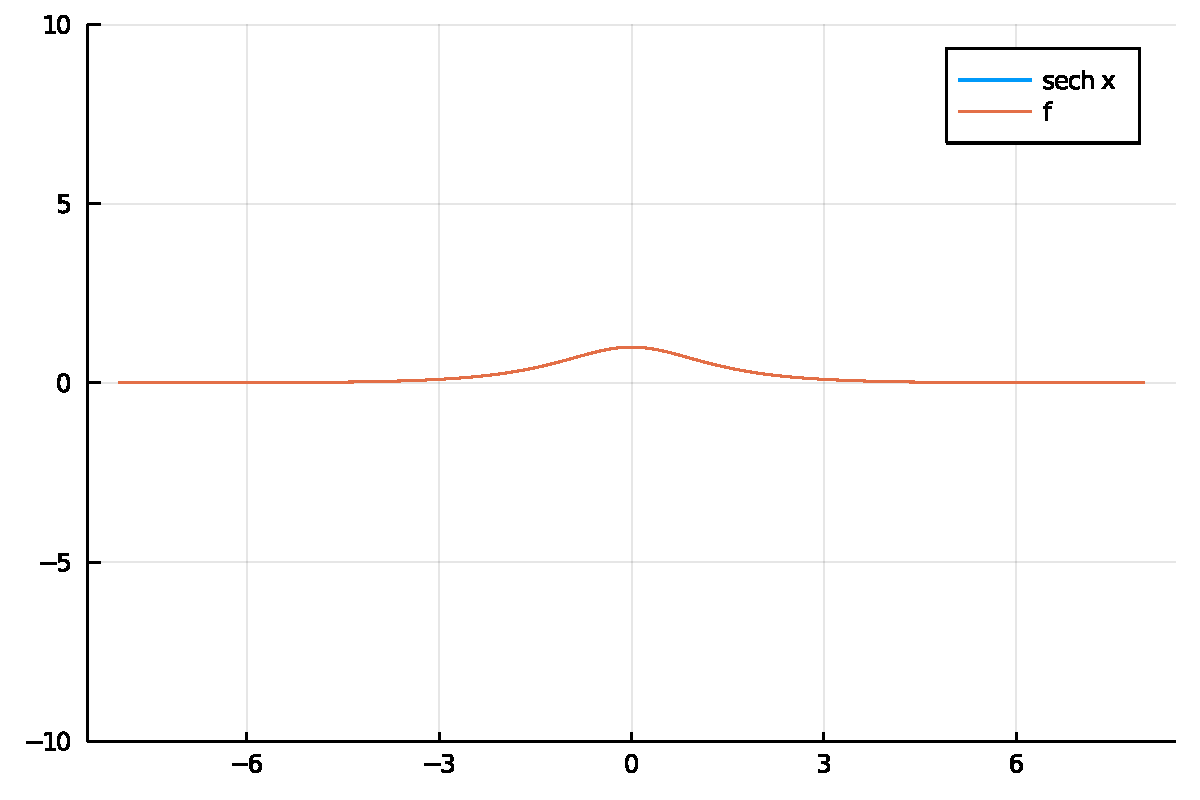
\includegraphics[width=\linewidth]{C:/Users/mfaso/OneDrive/Documents/GitHub/M3M6AppliedComplexAnalysis/output/figures/Lecture22_3_1.pdf}

Weighted by $w(x) = \E^{-x^2}$ breaks again:


\begin{lstlisting}
(*@\HLJLn{f}@*) (*@\HLJLoB{=}@*) (*@\HLJLnf{Fun}@*)(*@\HLJLp{(}@*)(*@\HLJLn{x}@*) (*@\HLJLoB{->}@*) (*@\HLJLnf{sech}@*)(*@\HLJLp{(}@*)(*@\HLJLn{x}@*)(*@\HLJLp{),}@*) (*@\HLJLnf{GaussWeight}@*)(*@\HLJLp{(}@*)(*@\HLJLnf{Hermite}@*)(*@\HLJLp{()),}@*)(*@\HLJLni{101}@*)(*@\HLJLp{)}@*)

(*@\HLJLnf{plot}@*)(*@\HLJLp{(}@*)(*@\HLJLn{xx}@*)(*@\HLJLp{,}@*) (*@\HLJLn{sech}@*)(*@\HLJLoB{.}@*)(*@\HLJLp{(}@*)(*@\HLJLn{xx}@*)(*@\HLJLp{);}@*) (*@\HLJLn{ylims}@*)(*@\HLJLoB{=}@*)(*@\HLJLp{(}@*)(*@\HLJLoB{-}@*)(*@\HLJLni{10}@*)(*@\HLJLp{,}@*)(*@\HLJLni{10}@*)(*@\HLJLp{),}@*) (*@\HLJLn{label}@*)(*@\HLJLoB{=}@*)(*@\HLJLs{"{}sech}@*) (*@\HLJLs{x"{}}@*)(*@\HLJLp{)}@*)
(*@\HLJLnf{plot}@*)(*@\HLJLp{(}@*)(*@\HLJLn{xx}@*)(*@\HLJLp{,}@*) (*@\HLJLn{f}@*)(*@\HLJLoB{.}@*)(*@\HLJLp{(}@*)(*@\HLJLn{xx}@*)(*@\HLJLp{);}@*) (*@\HLJLn{label}@*)(*@\HLJLoB{=}@*)(*@\HLJLs{"{}f"{}}@*)(*@\HLJLp{)}@*)
\end{lstlisting}

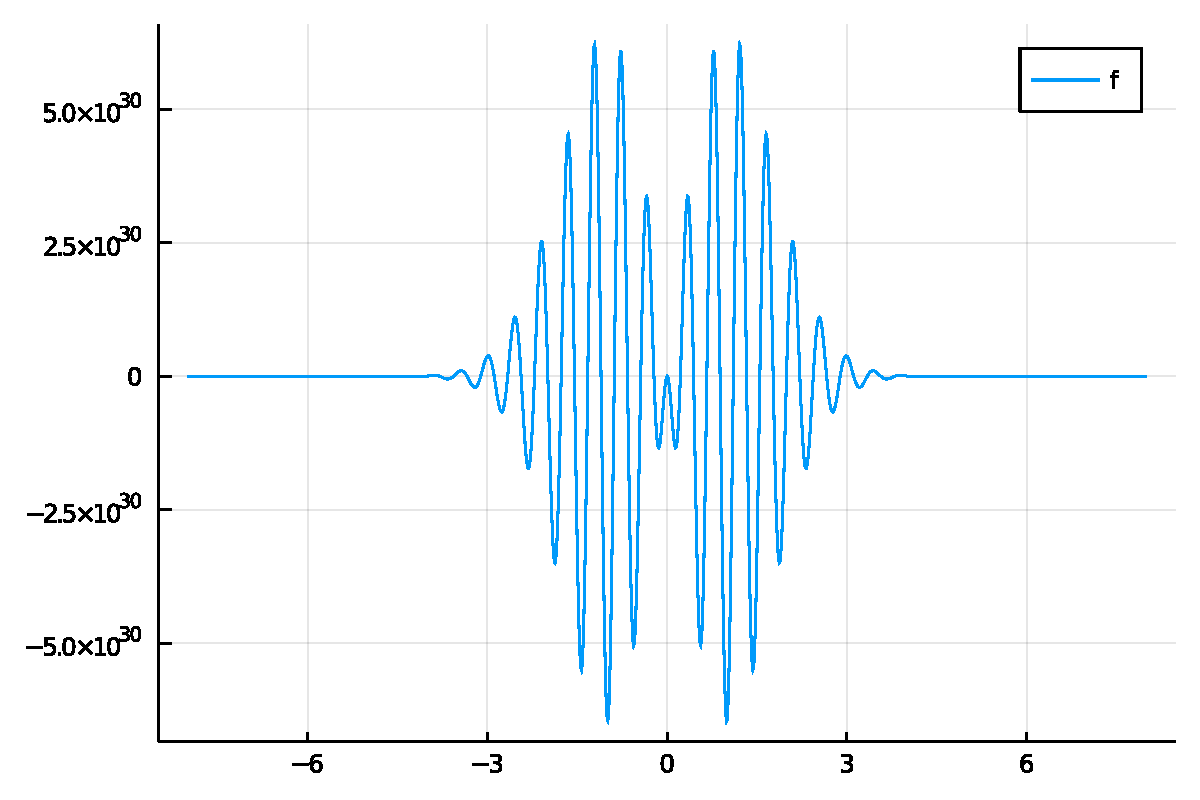
\includegraphics[width=\linewidth]{C:/Users/mfaso/OneDrive/Documents/GitHub/M3M6AppliedComplexAnalysis/output/figures/Lecture22_4_1.pdf}

This can be explained by observing that the functions

\[
\phi_k(x) = \E^{-x^2/2}H_k(x)
\]
are orthogonal in $L^2_{\mathbb{R}}$; the functions

\[
\widetilde{\phi}_k(x) = \E^{-x^2}H_k(x)
\]
are orthogonal in $L^2_{\mathbb{R}}(\E^{x^2})$; $\sech(x) \in L^2_{\mathbb{R}}$ but  $\sech(x) \notin L^2_{\mathbb{R}}(\E^{x^2})$. That is, the  $\phi_k(x)$ are orthogonal with respect to the weight $w(x) = 1$ on $\mathbb{R}$:

\[
\langle f, g \rangle_{w} = \int_{-\infty}^{\infty}f(x)g(x) \D x,
\]
the $\widetilde{\phi}_k(x)$ are orthogonal with respect to $\widetilde{w} = \E^{x^2}$:

\[
\langle f, g \rangle_{\widetilde{w}} = \int_{-\infty}^{\infty}f(x)g(x) \E^{x^2} \D x,
\]
for $f(x) = \sech(x)$, we have that

\[
\| f \|_{w}^2 = \langle f, f \rangle_{w} < \infty, \qquad \| f \|_{\widetilde{w}} = \sqrt{\langle f, f \rangle_{\widetilde{w}}} = \infty.
\]
Hence, $\sech(x)$ cannot have a convergent expansion of the form

\[
f(x) = \sum_{k = 0}^{\infty} f_k \widetilde{\phi}_k(x) = \E^{-x^2}  \sum_{k = 0}^{\infty} f_k H_k(x)
\]
in $L^2_{\mathbb{R}}(\E^{x^2})$ but it has an expansion in the functions $\phi_k(x)$ in $L^2_{\mathbb{R}}$. Obtaining bounds on the expansion coefficients $f_k$ in the functions $\phi_k(x)$ (as we did previously for Fourier expansions and Chebyshev expansions) is rather complicated and beyond the scope of this module.

\subsection{Application:  Eigenstates of Schrödinger operators with quadratic potentials}
Using the derivative formulae tells us a Sturm\ensuremath{\endash}Liouville operator for Hermite polynomials:

\[
\E^{x^2} {\D \over \dx} \E^{-x^2} {\D H_n \over \dx} = 2n \E^{x^2} {\D \over \dx} \E^{-x^2} H_{n-1}(x) = -2nH_n(x)
\]
or rewritten, this gives us

\[
{\D^2 H_n \over \dx^2} -2x {\D H_n \over \dx} = -2nH_n(x)
\]
We therefore have

\[
{\D^2 \over \dx^2}[\E^{-{x^2 \over 2}} H_n(x)] = \E^{-{x^2 \over 2}} (H_n''(x)  -2x H_n'(x) + (x^2-1) H_n(x)) = \E^{-{x^2 \over 2}} (x^2-1-2n) H_n(x)
\]
In other words, for the Hermite function $\psi_n(x)$ we have

\[
{\D^2 \psi_n \over \dx^2} -x^2 \psi_n = -(2n+1) \psi_n
\]
and therefore $\psi_n$ are the eigenfunctions.

We want to normalize.  In Schrödinger equations the square of the wave $\psi(x)^2$ represents a probability distribution, which should integrate to 1. Here's a trick: we know that

\[
x \underbrace{\begin{pmatrix} H_0(x) \\ H_1(x) \\ H_2(x) \\ \vdots \end{pmatrix}}_{\bm{H}} = \underbrace{\begin{pmatrix} 0 & {1 \over 2} \\
1 & 0 & \half \\
& 2 & 0 & \half \\
&& 3 & 0 & \ddots \\
&&& \ddots & \ddots
\end{pmatrix}}_J\begin{pmatrix} H_0(x) \\ H_1(x) \\ H_2(x) \\ \vdots \end{pmatrix}
\]
Let $\bm{H} = D^{-1}\bm{Q}$, where $D = \mathrm{diag}(d_0, d_1, \ldots)$ and $\bm{Q} = \left(q_0(x), q_1(x), \ldots \right)^\top$ denotes the (infinite) vector of orthonormal Hermite polynomials. We want to conjugate by $D$ so that $DJD^{-1}$ is symmetric because $x\bm{Q} = DJD^{-1}\bm{Q}$. We have

\[
DJD^{-1} = \begin{pmatrix}d_0 \\ & d_1 \\ &&d_2 \\&&&\ddots \end{pmatrix}  J \begin{pmatrix} d_0^{-1} \\ & d_1^{-1} \\ &&d_2^{-1} \\&&&\ddots \end{pmatrix} = \begin{pmatrix} 0 & {d_0 \over 2d_1} \\
{d_1 \over d_0} & 0 & {d_1 \over 2 d_2} \\
& {2d_2 \over d_1} & 0 & {d_2 \over 2 d_3} \\
&& {3d_3 \over d_2} & 0 & \ddots \\
&&& \ddots & \ddots
\end{pmatrix}
\]
We require:


\begin{align*}
d_1d_0^{-1} &= {d_0 \over 2 d_1} \Rightarrow d_1^2 = {d_0^2 \over 2} \\
2d_2d_1^{-1} &= {d_1 \over 2 d_2} \Rightarrow d_2^2 = {d_1^2 \over 4} = {d_0^2 \over 8} = {d_0^2 \over 2^2 2!} \\
3d_3d_2^{-1} &= {d_2 \over 2 d_3} \Rightarrow d_3^2 = {d_2^2 \over 3\times 2} = {d_0^2 \over 2^3 3!} \\
&\vdots \\
d_n^2 = {d_0^2 \over 2^n n!}.
\end{align*}
To determine $d_0$, note that $q_0 = d_0H_0 = d_0$ and thus

\[
\langle q_0, q_0 \rangle_{\rm H} =     d_0^2\int_{-\infty}^\infty \E^{-x^2} \dx = d_0^2\sqrt{\pi} = 1.
\]
Hence the orthonormal eigenfunctions in $L^2_{\mathbb{R}}$ with respect to the weight $w=1$ are

\[
    \psi_n(x) = q_n(x)\E^{-x^2/2} = d_n H_n(x)\E^{-x^2/2} = {H_n(x)\E^{-x^2/2}  \over \sqrt{\sqrt{\pi} 2^n n!} }
\]

\begin{lstlisting}
(*@\HLJLn{p}@*) (*@\HLJLoB{=}@*) (*@\HLJLnf{plot}@*)(*@\HLJLp{()}@*)
(*@\HLJLk{for}@*) (*@\HLJLn{n}@*) (*@\HLJLoB{=}@*) (*@\HLJLni{0}@*)(*@\HLJLoB{:}@*)(*@\HLJLni{5}@*)
    (*@\HLJLn{H}@*) (*@\HLJLoB{=}@*) (*@\HLJLnf{Fun}@*)(*@\HLJLp{(}@*)(*@\HLJLnf{Hermite}@*)(*@\HLJLp{(),}@*) (*@\HLJLp{[}@*)(*@\HLJLnf{zeros}@*)(*@\HLJLp{(}@*)(*@\HLJLn{n}@*)(*@\HLJLp{);}@*)(*@\HLJLni{1}@*)(*@\HLJLp{])}@*)
    (*@\HLJLn{\ensuremath{\psi}}@*) (*@\HLJLoB{=}@*) (*@\HLJLnf{Fun}@*)(*@\HLJLp{(}@*)(*@\HLJLn{x}@*) (*@\HLJLoB{->}@*) (*@\HLJLnf{H}@*)(*@\HLJLp{(}@*)(*@\HLJLn{x}@*)(*@\HLJLp{)}@*)(*@\HLJLnf{exp}@*)(*@\HLJLp{(}@*)(*@\HLJLoB{-}@*)(*@\HLJLn{x}@*)(*@\HLJLoB{{\textasciicircum}}@*)(*@\HLJLni{2}@*)(*@\HLJLoB{/}@*)(*@\HLJLni{2}@*)(*@\HLJLp{),}@*) (*@\HLJLoB{-}@*)(*@\HLJLnfB{10.0}@*) (*@\HLJLoB{..}@*) (*@\HLJLnfB{10.0}@*)(*@\HLJLp{)}@*)(*@\HLJLoB{/}@*)(*@\HLJLnf{sqrt}@*)(*@\HLJLp{(}@*)(*@\HLJLnf{sqrt}@*)(*@\HLJLp{(}@*)(*@\HLJLn{\ensuremath{\pi}}@*)(*@\HLJLp{)}@*)(*@\HLJLoB{*}@*)(*@\HLJLni{2}@*)(*@\HLJLoB{{\textasciicircum}}@*)(*@\HLJLn{n}@*)(*@\HLJLoB{*}@*)(*@\HLJLnf{factorial}@*)(*@\HLJLp{(}@*)(*@\HLJLnfB{1.0}@*)(*@\HLJLn{n}@*)(*@\HLJLp{))}@*)
    (*@\HLJLnf{plot!}@*)(*@\HLJLp{(}@*)(*@\HLJLn{\ensuremath{\psi}}@*)(*@\HLJLp{;}@*) (*@\HLJLn{label}@*)(*@\HLJLoB{=}@*)(*@\HLJLs{"{}n}@*) (*@\HLJLs{=}@*) (*@\HLJLsi{{\$}n}@*)(*@\HLJLs{"{}}@*)(*@\HLJLp{)}@*)
(*@\HLJLk{end}@*)
(*@\HLJLn{p}@*)
\end{lstlisting}

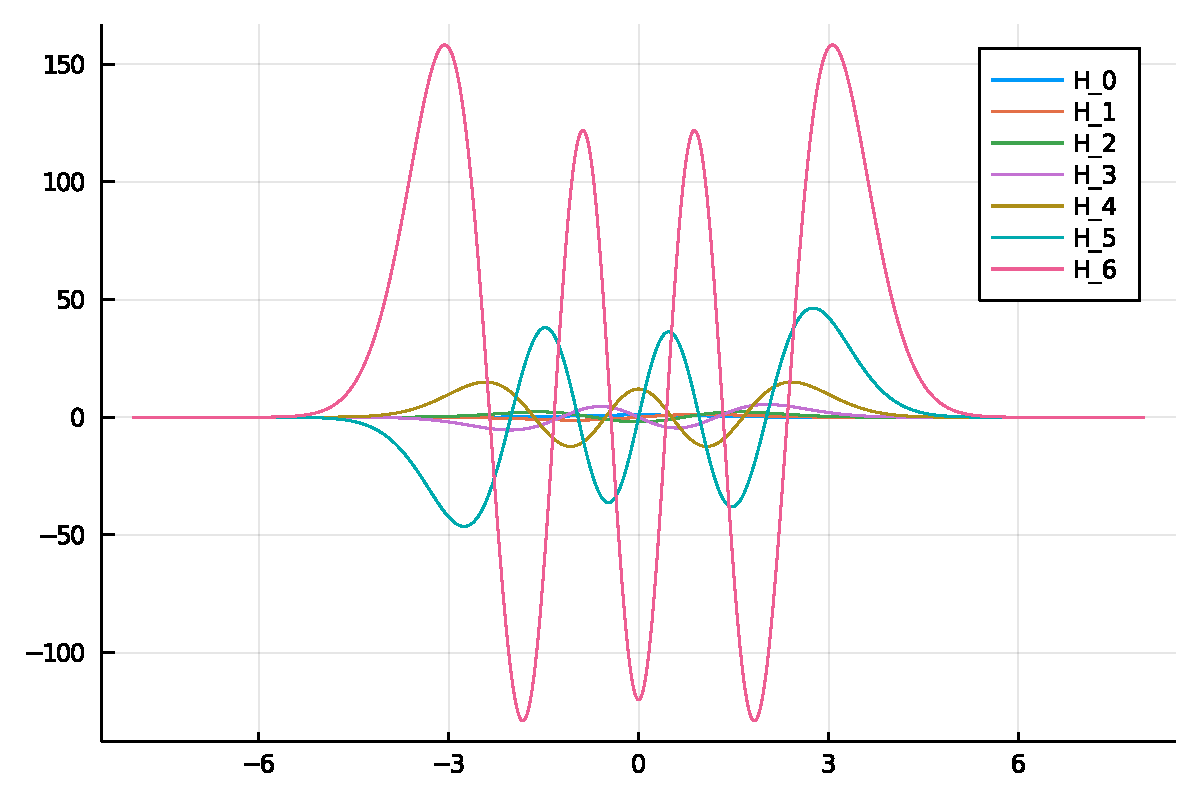
\includegraphics[width=\linewidth]{C:/Users/mfaso/OneDrive/Documents/GitHub/M3M6AppliedComplexAnalysis/output/figures/Lecture22_5_1.pdf}

It's convention to shift them by the eigenvalue:


\begin{lstlisting}
(*@\HLJLn{p}@*) (*@\HLJLoB{=}@*) (*@\HLJLnf{plot}@*)(*@\HLJLp{(}@*)(*@\HLJLnf{pad}@*)(*@\HLJLp{(}@*)(*@\HLJLnf{Fun}@*)(*@\HLJLp{(}@*)(*@\HLJLn{x}@*) (*@\HLJLoB{->}@*) (*@\HLJLn{x}@*)(*@\HLJLoB{{\textasciicircum}}@*)(*@\HLJLni{2}@*)(*@\HLJLp{,}@*) (*@\HLJLoB{-}@*)(*@\HLJLni{10}@*) (*@\HLJLoB{..}@*) (*@\HLJLni{10}@*)(*@\HLJLp{),}@*) (*@\HLJLni{100}@*)(*@\HLJLp{);}@*) (*@\HLJLn{ylims}@*)(*@\HLJLoB{=}@*)(*@\HLJLp{(}@*)(*@\HLJLni{0}@*)(*@\HLJLp{,}@*)(*@\HLJLni{25}@*)(*@\HLJLp{))}@*)
(*@\HLJLk{for}@*) (*@\HLJLn{n}@*) (*@\HLJLoB{=}@*) (*@\HLJLni{0}@*)(*@\HLJLoB{:}@*)(*@\HLJLni{10}@*)
    (*@\HLJLn{H}@*) (*@\HLJLoB{=}@*) (*@\HLJLnf{Fun}@*)(*@\HLJLp{(}@*)(*@\HLJLnf{Hermite}@*)(*@\HLJLp{(),}@*) (*@\HLJLp{[}@*)(*@\HLJLnf{zeros}@*)(*@\HLJLp{(}@*)(*@\HLJLn{n}@*)(*@\HLJLp{);}@*)(*@\HLJLni{1}@*)(*@\HLJLp{])}@*)
    (*@\HLJLn{\ensuremath{\psi}}@*) (*@\HLJLoB{=}@*) (*@\HLJLnf{Fun}@*)(*@\HLJLp{(}@*)(*@\HLJLn{x}@*) (*@\HLJLoB{->}@*) (*@\HLJLnf{H}@*)(*@\HLJLp{(}@*)(*@\HLJLn{x}@*)(*@\HLJLp{)}@*)(*@\HLJLnf{exp}@*)(*@\HLJLp{(}@*)(*@\HLJLoB{-}@*)(*@\HLJLn{x}@*)(*@\HLJLoB{{\textasciicircum}}@*)(*@\HLJLni{2}@*)(*@\HLJLoB{/}@*)(*@\HLJLni{2}@*)(*@\HLJLp{),}@*) (*@\HLJLoB{-}@*)(*@\HLJLnfB{10.0}@*) (*@\HLJLoB{..}@*) (*@\HLJLnfB{10.0}@*)(*@\HLJLp{)}@*)(*@\HLJLoB{/}@*)(*@\HLJLnf{sqrt}@*)(*@\HLJLp{(}@*)(*@\HLJLnf{sqrt}@*)(*@\HLJLp{(}@*)(*@\HLJLn{\ensuremath{\pi}}@*)(*@\HLJLp{)}@*)(*@\HLJLoB{*}@*)(*@\HLJLni{2}@*)(*@\HLJLoB{{\textasciicircum}}@*)(*@\HLJLn{n}@*)(*@\HLJLoB{*}@*)(*@\HLJLnf{factorial}@*)(*@\HLJLp{(}@*)(*@\HLJLnfB{1.0}@*)(*@\HLJLn{n}@*)(*@\HLJLp{))}@*)
    (*@\HLJLnf{plot!}@*)(*@\HLJLp{(}@*)(*@\HLJLn{\ensuremath{\psi}}@*) (*@\HLJLoB{+}@*) (*@\HLJLni{2}@*)(*@\HLJLn{n}@*)(*@\HLJLoB{+}@*)(*@\HLJLni{1}@*)(*@\HLJLp{;}@*) (*@\HLJLn{label}@*)(*@\HLJLoB{=}@*)(*@\HLJLs{"{}n}@*) (*@\HLJLs{=}@*) (*@\HLJLsi{{\$}n}@*)(*@\HLJLs{"{}}@*)(*@\HLJLp{)}@*)
(*@\HLJLk{end}@*)
(*@\HLJLn{p}@*)
\end{lstlisting}

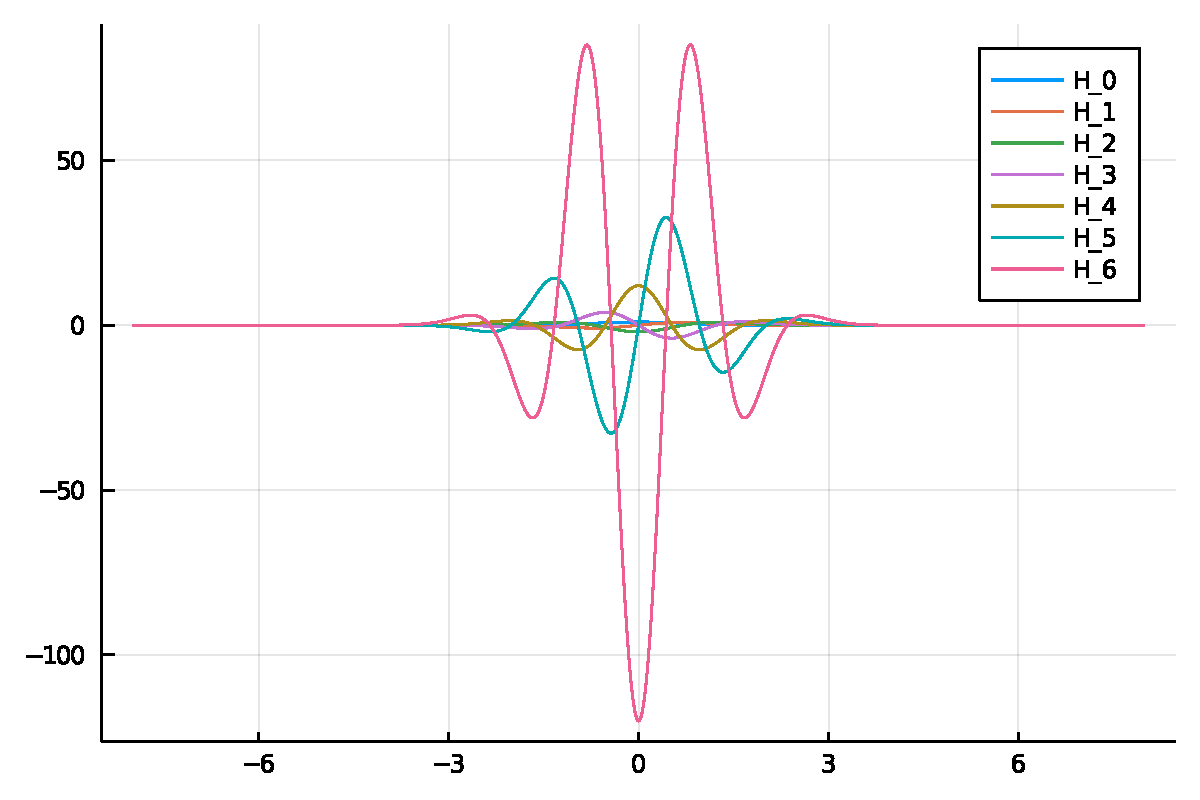
\includegraphics[width=\linewidth]{C:/Users/mfaso/OneDrive/Documents/GitHub/M3M6AppliedComplexAnalysis/output/figures/Lecture22_6_1.pdf}


\end{document}
